\documentclass{article}
\usepackage{tikz}

\renewcommand{\figurename}{Fig.}

\begin{document}

\begin{figure}[ht]
\centering

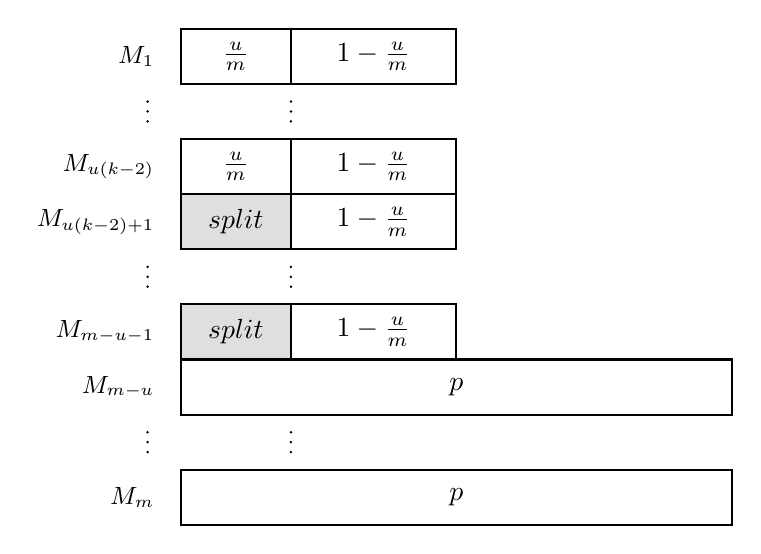
\begin{tikzpicture}[
    x=0.7cm,
    y=0.7cm,
    job/.style={
        draw,
        thick,
        fill=white,
        font=\small
    },
    machine/.style={font=\small}
]

% ------------------------------------------------
% Template idea:
% row      = displayed vertical row in the picture
% machine  = actual machine label shown on the left
%
% Use \machinerow{row}{machine label}
% Use \dotsrow{row}
% Use \jobblock{row}{start}{length}{job label}
% Use \jobblock[gray!25]{row}{start}{length}{job label} for shading
% ------------------------------------------------

\newcommand{\machinerow}[2]{
    \node[machine, anchor=east] at (-0.3,-#1+0.5) {$M_{#2}$};
}

\newcommand{\dotsrow}[1]{
    \foreach \dy in {-0.18,0,0.18} {
        \fill (-0.6,{-#1+0.5+\dy}) circle[radius=0.025];
        \fill (2,{-#1+0.5+\dy}) circle[radius=0.025];
    }
}

\newcommand{\jobblock}[5][white]{
    \draw[job, fill=#1] (#3,-#2) rectangle ++(#4,1);
    \node at ({#3 + #4/2},{-#2 + 0.5}) {$#5$};
}

% Displayed machine rows
\machinerow{1}{1}
\dotsrow{2}
\machinerow{3}{u(k-2)}
\machinerow{4}{u(k-2)+1}
\dotsrow{5}
\machinerow{6}{m-u-1}
\machinerow{7}{m-u}
\dotsrow{8}
\machinerow{9}{m}

% Example jobs
\jobblock{1}{0}{2}{\frac{u}{m}}
\jobblock{1}{2}{3}{1-\frac{u}{m}}

\jobblock{3}{0}{2}{\frac{u}{m}}
\jobblock{3}{2}{3}{1-\frac{u}{m}}

\jobblock[gray!25]{4}{0}{2}{split}
\jobblock{4}{2}{3}{1-\frac{u}{m}}

\jobblock[gray!25]{6}{0}{2}{split}
\jobblock{6}{2}{3}{1-\frac{u}{m}}
\jobblock{7}{0}{10}{p}
\jobblock{9}{0}{10}{p}

\end{tikzpicture}

\caption{Schedule structure showing full, split, and long processing blocks across selected machine rows.}
\label{fig:schedule-structure}

\end{figure}

\end{document}